% \subsubsection{Mô tả sitemap}
% Sitemap mô tả mối quan hệ phân cấp giữa các trang, luồng điều hướng logic, và phân nhóm chức năng theo module, giúp định hướng cho quá trình thiết kế giao diện và triển khai hệ thống.

% Cấu trúc được chia thành hai phần chính tương ứng với hai nhóm người dùng:
% \begin{itemize}
%     \item User App: dành cho người dùng cuối (Traveler, Guest, Provider).
%     \item Admin Portal: dành cho người quản trị và kiểm duyệt nội dung.
% \end{itemize}

% \begin{figure}[H]
%     \centering
%     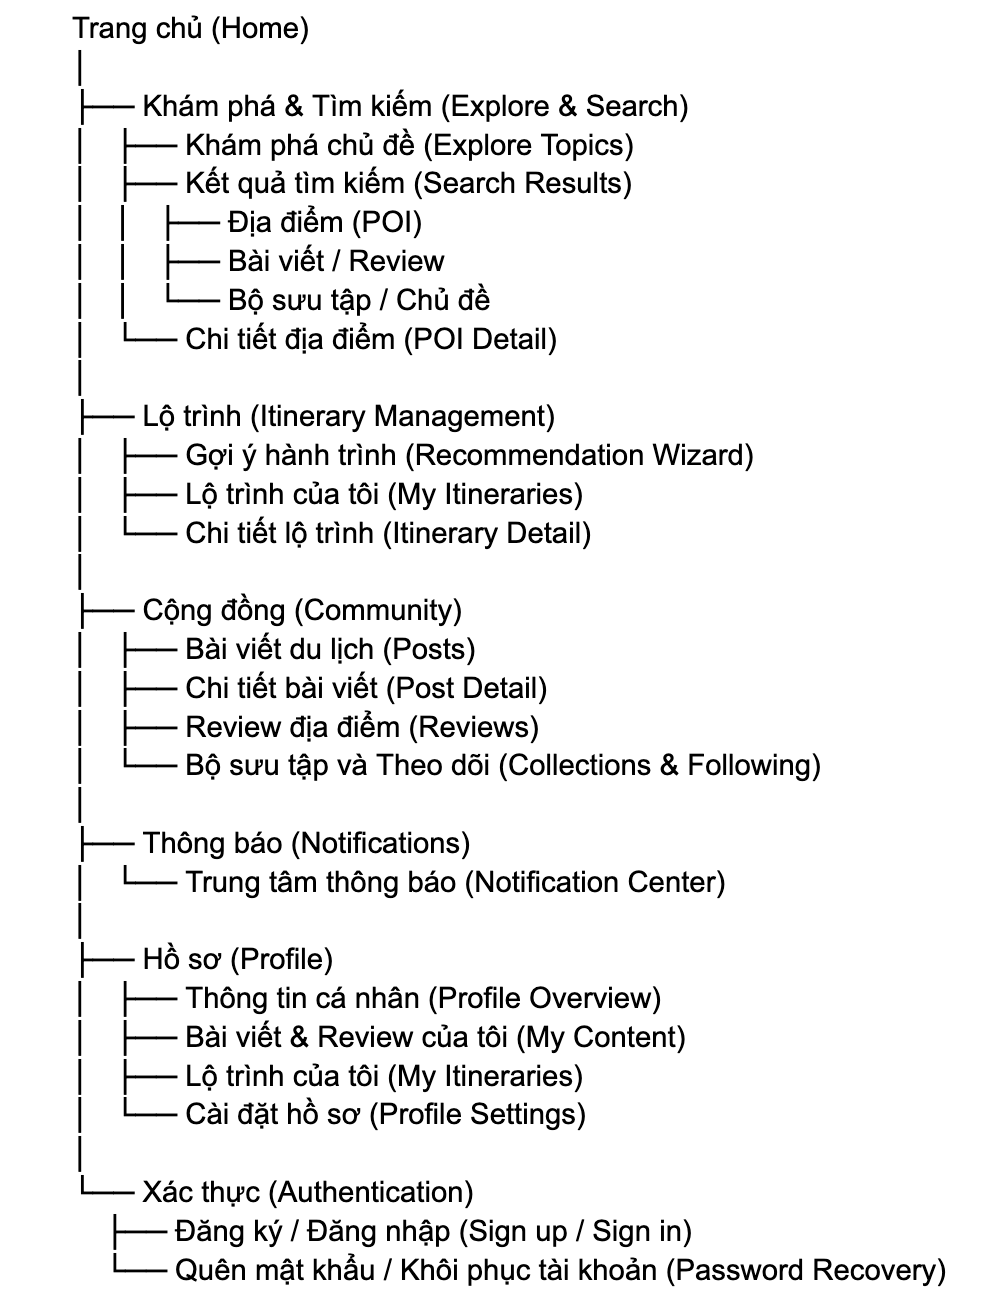
\includegraphics[width=1\textwidth]{Images/7. System Design/user.png}
%     \caption{Sitemap dành cho người dùng cuối}
%     \label{fig:sitemap_user}
% \end{figure}

% \begin{figure}[H]
%     \centering
%     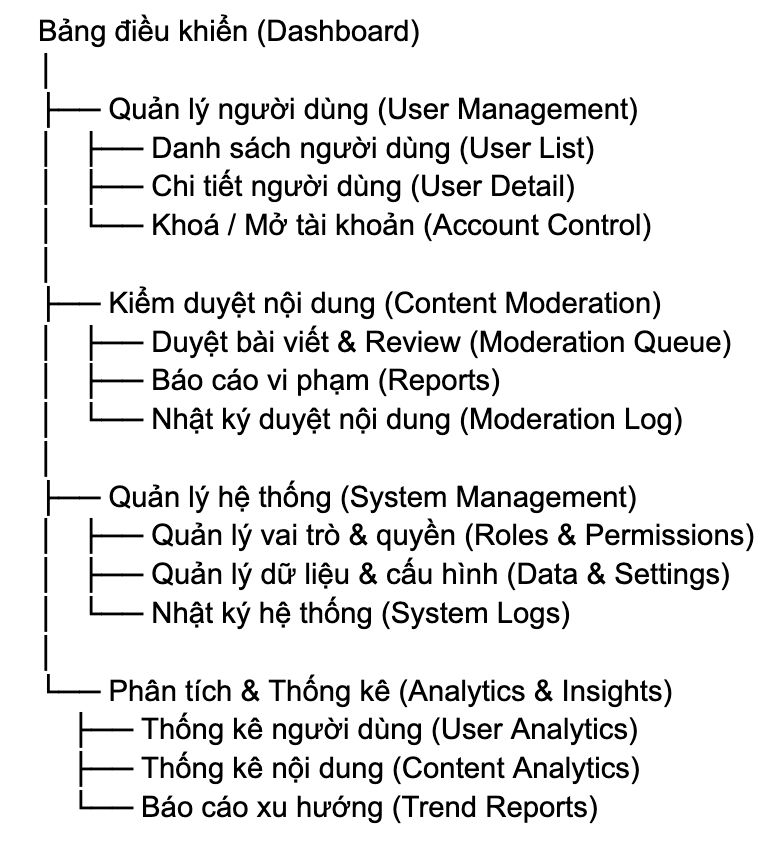
\includegraphics[width=1\textwidth]{Images/7. System Design/admin.png}
%     \caption{Sitemap dành cho quản trị viên}
%     \label{fig:sitemap_admin}
% \end{figure}
